\chapter{系统主要功能设计与实现}

\section{开发及运行环境}
\begin{enumerate}
	\item[(1)] 项目开发环境:
		\begin{itemize}
			\item CPU 最低Intel Core i5 4590或同等性能芯片。
			\item 推荐 Intel Core i7 7700或AMD同等性能芯片及以上。
			\item 内存 最低8GB(推荐16GB及以上)。
			\item 硬盘 需要10GB以上的可用空间(固态硬盘为宜)。
			\item 网络 接入互联网下行20Mbps及以上,上行10Mbps及以上。
			\item 操作系统 macOS Big Sur Version 11.3.1。
			\item 基本软件 JDK-11、MariaDB、Redis、ElasticSearch和Maven。
		\end{itemize}
	\item[(2)] 软件部署环境:
		\begin{itemize}
			\item CPU 最低Intel Core i5 4590或同等性能芯片。
			\item 推荐 Intel Core i7 7700 或AMD同等性能芯片及以上。
			\item 内存 最低8GB(推荐16GB及以上。
			\item 硬盘 需要10GB以上的可用空间(固态硬盘为宜)。
			\item 网络 接入互联网下行20Mbps及以上,上行10Mbps及以上。
		\end{itemize}
\end{enumerate}

\section{系统架构设计}
系统采用B/S(Browser/Server,浏览器/服务器)方式的网络结构,统一采用如Chrome一类的浏览器,通过访问前端服务器获取页面,
前端服务器通过Json向业务服务器发送请求,由Nginx负载均衡分发给各个业务服务器,业务服务器对请求处理后,将结果返回给客户端。
架构设计如图\ref{figure:jiagou}所示。
\begin{figure}[!htbp]
\centering
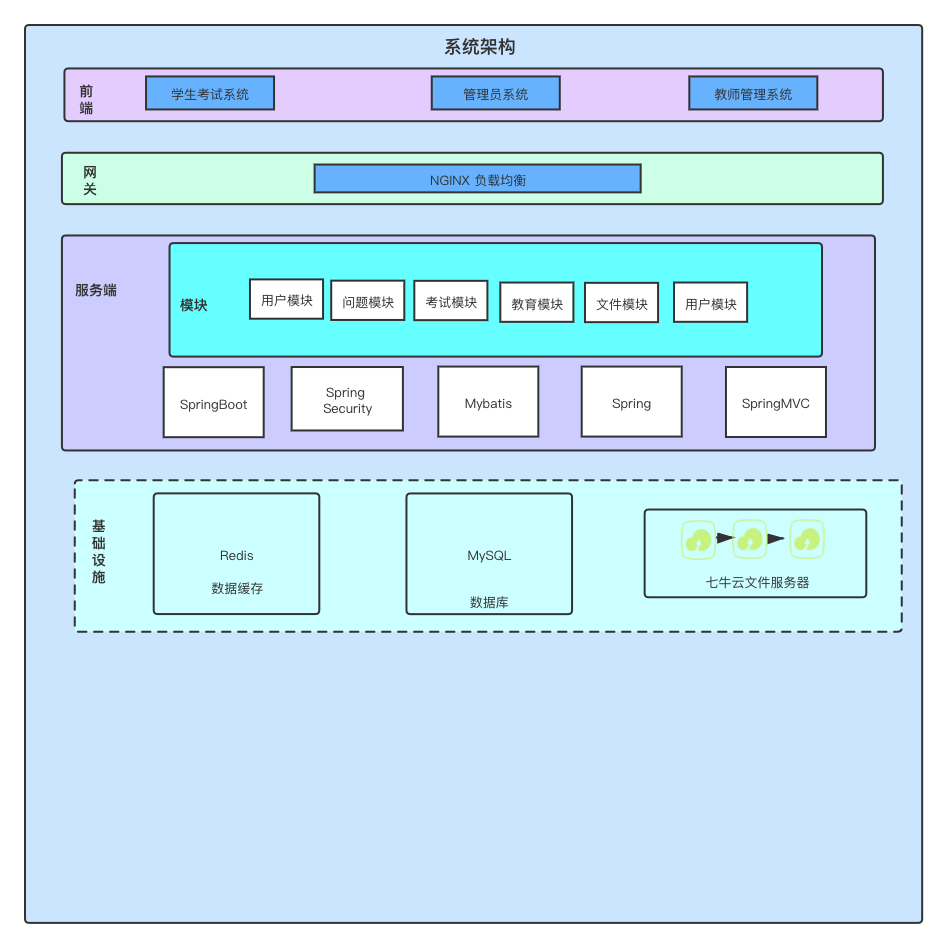
\includegraphics[width=0.6\textwidth,keepaspectratio]{data/chapter-2/jiagou.png}
\caption{系统架构}
\label{figure:jiagou}
\end{figure}

\section{系统各个功能模块的分析与设计}
在线考试系统分为学生、老师和管理员三个子系统。学生端主要功能是进行在线测试并可以查看以往的错题,老师端可以进行试题的管理和考试的安排,管理员可以对用户进行管理、试题管理和考试的全部安排。
\subsection{学生端}
\begin{enumerate}
	\item[(1)] 练习和考试模块:\\
	学生访问通过主面板的相关考试入口,可以通过固定试卷和时段试卷练习,固定试卷是老师发布一直为提供练习的试卷,时段试卷是老师发布的暂时为学生提供练习。可以通过任务中心进行考试。考试开始后,需要打开摄像头
考试期间将随机进行拍照监控并将照片上传至图片服务器。考试完成后,将自动批阅客观题目,并给出客观题目总得分。
	\item[(2)] 错题本模块:\\
	学生在考试或者练习并且当试卷评分完成后,可以在错题本模块查看自己的历史错题,所有做错的题目,可以看到做题的结果、分数、难度、解析、正确答案等。
	\item[(3)] 考试记录模块:\\
	在考试模块,学生可以查看历史的考试记录,其中包括考试的用时、状态和分数。
	\item[(4)] 个人信息模块:\\
	学生在个人信息模块可以进行个人基本信息的修改和密码的修改。
\end{enumerate}
\begin{figure}[!htbp]
\centering
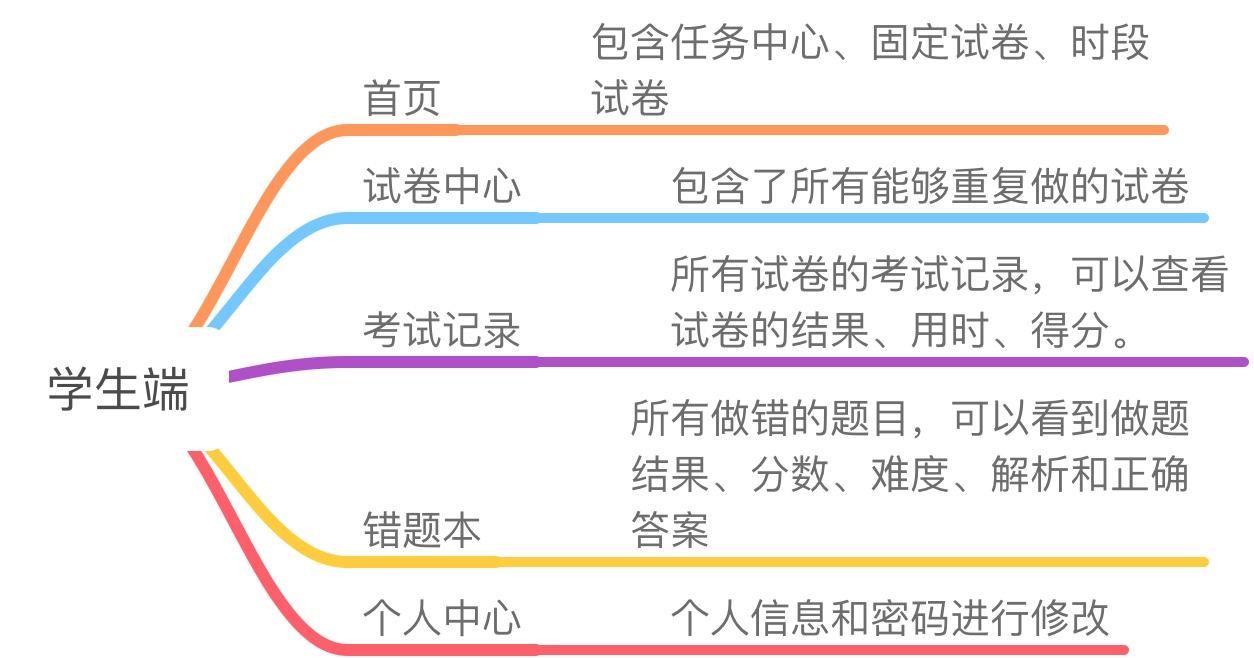
\includegraphics[width=0.6\textwidth,keepaspectratio]{data/chapter-3/xueshengduan.png}
\caption{学生端各个模块}
\label{figure:student}
\end{figure}


\subsection{教师端}
\begin{enumerate}
	\item[(1)] 学生管理:\\
	学生管理模块中,来时可以强制修改本班学生的个人信息和密码。
	\item[(2)] 试卷模块:\\
	老师可以通过试卷模块向题库中添加试题,同时老师也可以设计自己的试卷。
	\item[(3)] 教育管理和任务管理:\\
	在教育管理中老师可已进行发布练习试卷和查看学生们的练习情况,在任务管理中老师可以发布考试。
	\item[(4)] 答卷模块:\\
	在答卷模块中老师可以查看本班级的所有答卷记录,并批改主观题目给出得分。
\end{enumerate}
\begin{figure}[!htbp]
\centering
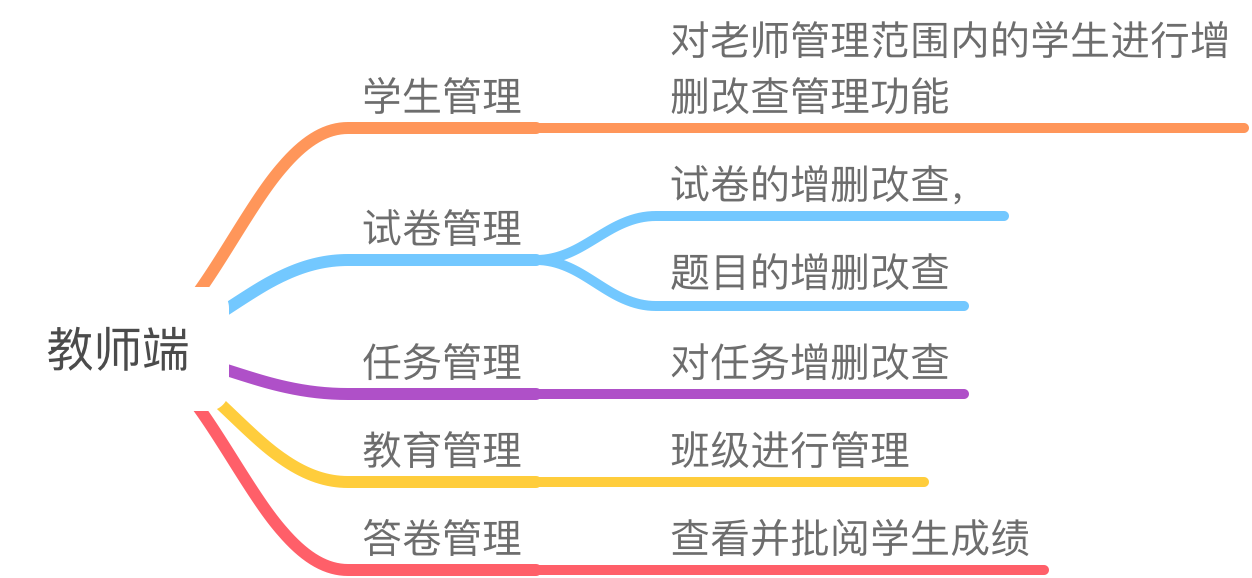
\includegraphics[width=0.6\textwidth,keepaspectratio]{data/chapter-3/jiaoshiduan.png}
\caption{教师端的各个模块}
\label{figure:teacher}
\end{figure}

\subsection{管理员端}
管理员端相当于权限大一些的老师,老师的管理范围是自己所属的班级,而管理员的管理范围则是整个系统中的所有用户。
\begin{figure}[!htbp]
\centering
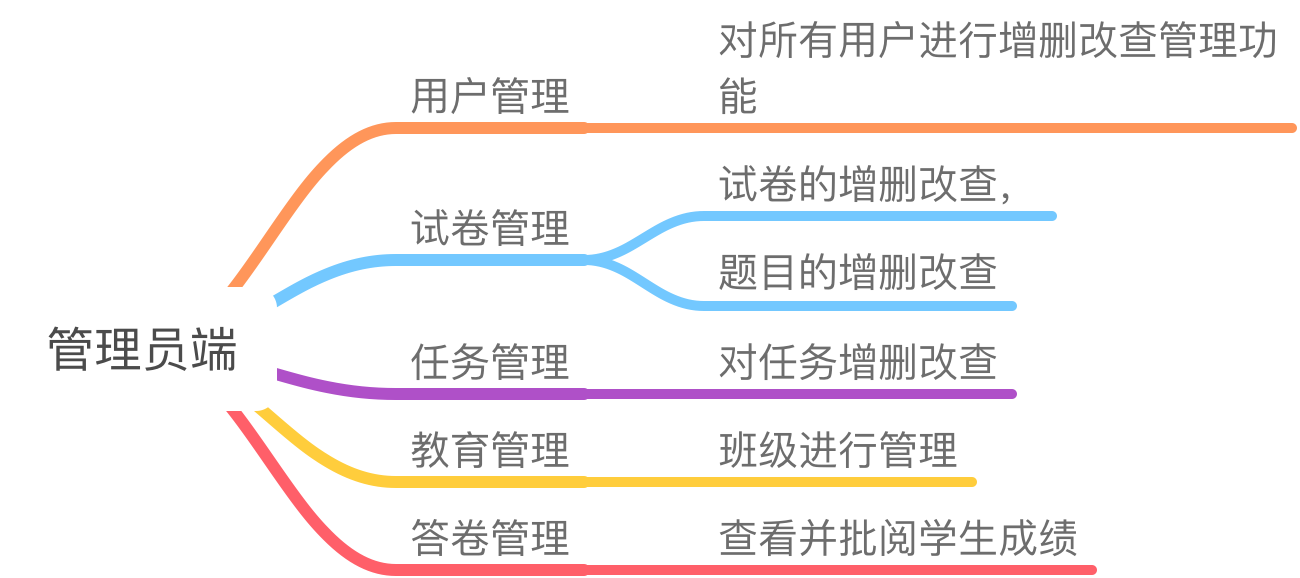
\includegraphics[width=0.6\textwidth,keepaspectratio]{data/chapter-3/admin.png}
\caption{管理员端的各个模块}
\label{figure:teacher}
\end{figure}